\documentclass{article}

%%--LANGUAGE AND ENCODING--%%
\usepackage[swedish]{babel}
\usepackage[english,cleanlook]{isodate}%
\usepackage[utf8]{inputenc}
\usepackage{csquotes}

\usepackage[yyyymmdd]{datetime}
\renewcommand{\dateseparator}{--}

%%--BIBLOPGRAPHY--%%
\usepackage[natbib=true, style=ieee,  backend=biber, dateabbrev=false, urldate=iso8601, maxbibnames=4]{biblatex} %style=authoryear, citestyle=authoryear, maxcitenames=2,


%%--SPACING AND MARGIN--%
\usepackage[margin=4cm, top=2.5cm]{geometry}

%%--SANS-SERIF FONTS FOR SECTIONS--%%
\usepackage{sectsty}
\usepackage{helvet}
\allsectionsfont{\bfseries\sffamily}

%%Links within the doc%%
\usepackage[hidelinks]{hyperref}
%%--GRAPHICS--%%  (Requires preamble)
% \usepackage{tikz}
\usepackage{graphicx}
\usepackage{caption}
\usepackage[justification=centering]{caption}
\usepackage{subcaption}


%%--ADVANCE TABULARS--%%
 \usepackage{tabularx}
\def\arraystretch{1.3}
%PREAMBLE%
%%-SECTION NUMMBERING DEPTH-%%
%\setcounter{secnumdepth}{3} %3=Default

%%-GRAPHICS-%%
\DeclareGraphicsExtensions{.pdf,.png,.jpg}


%%-BIBLIOGRAPHY-%%
%Adds references library and formats it.
% To  refere to a reference in the library use  \cite{} for ieee
%                                               \citep{} for authoryear
\addbibresource{ref.bib} \setlength{\bibitemsep}{\baselineskip} 
%Always shows the authors in bibliography as Lastname, Firstname
%\DeclareNameAlias{sortname}{last-first} 

%%-DOCUMENT INFORMATION-%%
%Header/Footer%
\author{    Strand, Johan \\ \texttt{johstr@student.chalmers.se} \\ 
            19870101--4899 \and
            Svedberg, Pär\\ \texttt{svpar@student.chalmers.se}  \\ 
            19821112--7652 \and
            Åkergren, Oskar\\ \texttt{akergren@student.chalmers.se}  \\ 19880505--7114
}
\title{\vspace{2cm} Styrdosa till \\ Parans solpanel  \vspace{1cm}}

\date{\vspace{8cm}\today}

\begin{document}
    \maketitle
    \thispagestyle{empty}

    \newpage 
    \subsection*{Abstract (draft)} % (fold)
    \label{sub:abstract}
            The purpose of this research was to find an alternative and more user friendly way of installing and controlling a sun panel manufactured by Parans Solar Lightning. \\

            \noindent Today is the panel installed and controlled by connecting a computer to the panel which have to be correctly configured and able to run a terminal where commands are sent to the panel.\\

            \noindent This research where done in co-operation with Parans Solar Lightning and the aim was to develop a hand held device which is easy to connect and has buttons that executes the commands needed to install and controll the panel.\\

            \noindent The resulting device is a GUI devoloped in python, with tkinter as GUI-library, running on a Raspberry Pi with an attached touchscreen. The device is connected to the panel via an USB cable and the user controls the panel by pressing simple (maybe informal..) buttons on the touchscreen.\\

            \noindent The result provide a solution for Parans which they can take in to further development and sell to their customers as an easy way of installing and controlling the sun panel.
    % subsection beteckningar(end)

    \newpage 
    \subsection*{Beteckningar} % (fold)
    \label{sub:beteckningar}
        \begin{tabularx}{\textwidth}{@{}lX}
            C & Imperativt programmeringsspråk \\
            CP2102 & Enhet från Silicon Labs som omvandlar kommunikation från
            USB till seriell enligt RS232\\
            GUI & Graphical User Interface, grafiskt användargränssnitt \\
            I/O & Input/Output \\
            PIC32 & 32-bitars mikrokontroller \\
            Python & Högnivåspråk för programmering \\
            SP3 & Parans solpanel, tredje generationen \\
            SSH & Secure Shell. Protokoll för säker anslutning mellan datorer\\
            USB & Universal Serial Bus, standard för seriell kommunikation \\
            \\
            Enkortsdator & I denna rapport menas enkortsdatorer av typen System
            on a chip, exempelvis enheter från Raspberry Pi och Beagle\-bone. 
            En enkortsdator ska enligt rapportens definition klara av att driva 
            operativsystem innehållande Linuxkärnan eller mot\-svarande. \\
            Mikrokontroller & Här menas enchipdatorer avsedda att programmeras 
            direkt till enhetens programminne, exempelvis enheter från 
            \hbox{Arduino}. Dessa klarar ej av att driva operativsystem 
            innehållande Linux\-kärnan eller motsvarande.\\
            

        \end{tabularx}
    % subsection beteckningar(end)
    \newpage

    \tableofcontents

    \newpage

    \section{Introduktion} % (fold)
    \label{sec:introduktion}
    % section section_name (end)

        \subsection{Bakgrund} % (fold)
        \label{sub:bakgrund}
            Parans har utvecklat en produkt som via optiska fibrer levererar naturligt solljus. Som ett av få bolag i världen levererar de system globalt och deras för närvarande största installationer finns i Malaysia och Los Angeles.\\

            \noindent Med hjälp av linser fokuseras solljus in i optiska fibrer och panelen styrs med hjälp av två stegmotorer. Styrningen sker på input dels från en algoritm som, baserat på position (longitud, latitud) och tid, ger en solposition i grader och dels från en solsensor med fotocell som ger data för en finstyrning av panelens positionering då solen är framme. Detta för att alltid maximera solljusets fokusering in i fibern.\\

            \noindent Själva panelen körs på 12V och dess systemdesign bygger på en PIC32; koden är skriven i C. Parans kommunicerar med enheten via USB--port och en terminalemulator. 
        % subsection bakgrund (end)
        
        \subsection{Syfte} % (fold)
        \label{sub:syfte}
            Idag styrs panelen till rätt position via en terminalemulator, vilket är en tröskel för Parans kunder vid installation och felsökning.  Exempelvis har alla inte vana av att jobba i terminaler och det kan vara krångligt att konfigurera datorns USB--portar så att kommunikation kan ske med panelen. \\

            \noindent Parans vill därför utveckla en styrdosa/box med tryckknappar, lysdioder och eventuellt en display som minskar problemen för kunderna. Denna box kan vara i form av ett befintligt kort som t.ex. Raspberry Pi, Arduino eller liknande men skulle också kunna vara en app för Android/iOS som kan köras på en kundens mobila enhet.
        % subsection syfte (end)

        \subsection{Frågeställning} % (fold)
        \label{sub:fragestallning}
        Rapporten ämnar att besvara följande frågeställningar:
        \begin{itemize}
            \item Vad styr valet av plattform för styrdosan?
            \item Vilken plattform blir enklast för kunderna att använda?
            \item Påverkar valet av plattform huruvida styrdosan blir kompatibel med framtida versioner av solpanelen?
            \item Vilket programmeringsspråk lämpar sig bäst för styrdosan?
        \end{itemize}   
        

        % subsection fr_gest_llning (end)

        \subsection{Avgränsning} % (fold)
        \label{sub:avgransning}
            Vi ser att detta projekt kommer kunna skapas med existerande hårdvara i form av mikrokontrollerkort, telefoner eller enkortsdatorer. Detta ger att vi kommer att begränsa projektet till dessa former och inte utveckla ett eget mönsterkort.\\

            \noindent Dagens paneler kan kommunicera med externa enheter via en USB--port men saknar övriga kommunikationsmöjligheter i dagsläget. Detta gör att projektet begränsas till kommunikation via en ansluten USB--kabel och inte via någon trådlös kommunikation.
        % subsection avgr_nsning (end)

    \section{Metod} % (fold)
    \label{sec:metod}

        Vi har för detta projekt valt jobba utifrån undersökningsmetoden beskriven i \\
        ''A design science research methodology for information systems research'' \cite{method}. \\

        \noindent Metoden Design Science Research (DSR) beskriver efterforskning uppdelad i fem faser;
        \textit{Problem Analysis \& Motivation, Design \& Development, Demonstration, Evaluation} and \textit{Communication}. 
        I den första fasen identifieras problemområdet tillsammans med Parans och vilken lösning som efterfrågas. I faserna \textit{Design \& Development, Demonstration and Evaluation} tar vi fram en prototyp som i varje iteration utvärderas för att se hur den väl den uppfyller de krav som sattes upp.
        Resultat presenteras slutligen i fasen \textit{Communication} som dels en muntlig presentation och dels en skriven rapport. \\

        \noindent En alternativ metod till DSR är 'Action Research' (AR) vars mål är att iterativt lösa ett problem med hjälp av en grupp av definierade metoder \cite{actionresearch}. AR är väldigt lik DSR i sitt utförande \cite{designscience} och båda metoderna skapar om kunskap om specifika situationer och problem. Anledningen att valet föll på DSR var att metoden strävar mot att att designa och skapa artefakter vilket går väl ihop med projektet om att utveckla en handhållen fysisk enhet. 
        Med artefakt menas i det här sammanhanget en prototyp som evalueras hur väl den löser ett uppsatta problem. 

    \newpage

    \section{Genomförande} % (fold)
    \label{sec:genomforande}
        Detta avsnitt avser behandla projektets utförande enligt den i föregående avsnitt beskrivna metoden DSR.
        
        \subsection{Problemanalys} % (fold)
        \label{sub:problemanalys}
            Parans vision var att utveckla en mobil, handhållen enhet som via seriell kommunikation kan kommunicera med och agera fjärrkontroll till solpanelen SP3.  I ett inledande skede diskuterades tekniska lösningar och vilka funktioner som var önskvärda från bolagets sida. Dessa funktioner var indelade i ett grundutförande och två nivåer av extrafunktioner. \\
            
            \noindent Grundutförandet innehöll funktioner för att kunna skicka styrkommandon i syfte att justera panelen vertikalt och horisontellt, omstart, läsa av tids- och geopositionsinställningar och att kunna försätta panelen i installationsläge. \\
            
            \noindent Extrafunktionerna innebar att ansluta en GPS-modul till fjärrkontrollen. Den första nivån av extrafunktioner var att kunna verifiera panelens geoposition medan den andra nivån bestod av att i panelen kunna ställa in tids-- och geopositionsuppgifter, bägge med hjälp av information givet av GPS-modulen. Projektets mål var att inom den givna tidsramen utveckla en fjärrkontroll enligt grundutförande och om tid återstod efter detta att påbörja implementation av extrafunktioner.
        % subsection problemanalys (end)

        \subsection{Design och utveckling} % (fold)
        \label{sub:design_och_utveckling}
        
            \subsubsection{Val av plattform} % (fold)
            \label{subsub:val_av_plattform}
            För att kunna konstruera den typ av fjärrkontroll som möter projektets krav var först ett beslut tvunget att tas om vilken teknisk plattform som skulle användas. De alternativ som diskuterades var Androidbaserade enheter, Arduinosystem och enkortsdatorer, främst Raspberry Pi.\\
            
            \noindent Egenskaper som beaktades var utvecklingskomplexitet, användarvänlighet, kostnad och kompatibilitet med SP3s enhet för seriell kommunikation, CP2102. USB-anslutningar kräver att en av enheterna agerar värd (eng. 'host') och för att kunna kommunicera seriellt till CP2102 behöver plattformen ha stöd för 'USB-host', då SP3 saknar stöd för detta. \\
            
            \noindent Bland Androidenheter sågs fördelar i att de har en färdigutvecklad produkt innehållande pekskärm, komplett datorsystem, integrerat batteri och att drivrutiner finns tillgängliga till CP2102. Nackdelar var att de är relativt dyra, information om vilka enheter som stöder USB-host är bristfällig och att för att använda drivrutinen till CP2102 krävs i de allra flesta fall att denna integreras manuellt i en egenbyggd Androiddistribution \cite{SL_AN809}. \\
            
            \noindent Arduino och Raspberry Pi har till viss del gemensamma fördelar och nackdelar. Båda plattformarna har stöd för USB-host, tillgång till mycket information då de är populära bland entusiaster och att det finns många utbyggnadsmoduler. Vad som kan ses som negativt är att ingendera levereras med skärm eller tryckknappar och att enheten kan bli otymplig vid anslutning av flera tilläggsmoduler. En fördel Arduino har gentemot Raspberry Pi är att den förstnämnda har lägre energiförbrukning medan den sistnämnda har drivrutiner till CP2102 integrerade i Linuxkärnan. Till Arduino måste alltså en drivrutin först programmeras. \\


            \noindent\textsf{\textbf{Androidenhet}}\\
            \begin{tabularx}{\textwidth}{@{}cXcX}
                & \textbf{Fördelar}     & & \textbf{Nackdelar} \\
                $+$ & Pekskärm medför stor valfrihet i utförande av användargränssnitt     &                            $-$ & Otydligt vilka enheter som
                                                  stöder USB-host \\
                $+$ &  Etablerat OS     &   $-$ & Relativt dyr \\
                $+$ &  Stor skärmyta    &   $-$ & Mer prestanda än nödvändigt \\
                $+$ &  Drivrutiner till CP2102 existerar &
                                            $-$ & Kräver egenbyggd Androiddistribution \\
            \end{tabularx}\\

                
            \noindent\textsf{\textbf{Raspberry Pi}}\\
            \begin{tabularx}{\textwidth}{@{}cXcX}
                & \textbf{Fördelar}     & & \textbf{Nackdelar} \\
                $+$ & God tillgång till information & 
                                        $-$ & Mer prestanda än nödvändigt \\
                $+$ & God tillgång till utbyggnads\-moduler & 
                                        $-$ & Saknar skärm och knappar i 
                                              grundutförande \\
                $+$ & Drivrutiner till CP2102 i Linuxkärnan &
                                        $-$ & Kan bli otymplig vid användande av   
                                              många tilläggsmoduler \\   
                $+$ & Lågt pris \\   
            \end{tabularx}\\
            
            \noindent\textsf{\textbf{Arduinosystem}} \\ 
            \begin{tabularx}{\textwidth}{@{}cXcX} 
                & \textbf{Fördelar}     & & \textbf{Nackdelar} \\
                $+$ & God tillgång till information & 
                                        $-$ & Saknar skärm och knappar i 
                                            grundutförande \\
                $+$ & God tillgång till utbyggnads\-moduler & 
                                        $-$ & Otymplig vid användande av   
                                            många tilläggsmoduler \\
                $+$ & Låg energiförbrukning &
                                        $-$ & Saknar drivrutiner till CP2102 \\

            \end{tabularx}
            % subsubsection val_av_plattform (end)

            \subsubsection{Mjukvaruutveckling} % (fold)
            \label{subsub:mjukvaruutveckling}
            För att erbjuda användaren ett användargränssnitt som är lättanvänt och fungerar väl ihop med en pekskärm så lades fokus på att implementera ett gränssnitt med stora tydliga tryckknappar. Då skärmens yta är begränsad beslutades att inte ha lägga all funktionalitet i en vy utan att separera den del som manövrerar solpanelen från den del som skickar kommandon för avläsning, automatisering och omstart. Detta minskar risken för att trycka på fel knapp och därmed sätta panelen i ett oönskat läge.\\

            \noindent När panelen kontrolleras via en terminal får användaren feedback från panelen genom att statusmeddelanden skrivs ut i terminalen. 
            Dessa meddelanden valde vi att presentera i ett statusfält placerat i botten på pekskärmen och som är tillgängligt oavsett vy.\\

            \noindent För att ansluta till solpanelen krävs, förutom en fysisk anslutning USB-kabel, även att en seriell anslutning upprättas. Denna anslutning kan antingen upprättas automatiskt genom att programmet ligger och läser av om något är anslutet till fjärrkontrollens USB-port eller att användaren gör ett aktivt val genom att trycka på en knapp.\\
            %Osäker på huruvida jag bör skriva vad vi implementerade under mjukvaruutveckling. Tillhör egentligen resultdelen?

            % subsubsection mjukvaruutveckling (end)

            
            Linuxsystemet på den enkortsdator som tillhandahölls av bolaget, ett utvecklingskort från Olimex, behövdes initialt konfigueras för att möjliggöra SSH--anslutning via nätverk. För detta användes en USB-till--seriell--kabel kopplad mellan utvecklings\-kortets seriella pinkontakter och en persondators USB--port. Seder\-mera anslöts enkortsdatorn via en nätverksbrygga till bolagets trådlösa nätverk och SSH--anslutningen verifierades. Ett första test för att säkerställa att kommunikation mellan enkortsdatorn och SP3 kunde upprättas utfördes genom att koppla samman enheterna med en USB--kabel. Utvecklings\-kortets Linuxsystem identifierade automatiskt anslutning av SP3s CP2102 och denna monterades automatiskt i \hbox{Linux} som \texttt{/dev/ttyUSB0}. Med hjälp av ett terminal\-program kunde kommandon skickas till SP3, som i sin tur utförde dessa och svarade korrekt.
        % subsection design_och_utveckling (end)

    % section genomforande (end)

    \newpage

    \section{Resultat} % (fold)
    \label{sec:resultat}
        Det här avsnittet avser att knyta an till frågeställningen och besvara de frågor som ligger till grund för arbetet. Resultatet presenteras genom en redovisning av den produkt som genomförandet har lett fram till. \\

        \noindent Resultatet av genomförandet är en handhållen produkt som kopplar in sig till sol\-panel\-en via en USB--sladd, där grunden i enheten är en 'Raspberry Pi' och användargränssnittet består av en resistiv pekskärm framtagen till just denna plattform \cite{Ada}. Produkten placeras i ett inköpt chassi framtaget för att husera just denna konfiguration. Enheten strömförsörjs genom ett batteripaket även det inhandlat från återförsäljare, ett batteripaket som är framtaget för att agera laddare för laddnings enhet för enheter som laddas via USB, men det visade sig vara lämplig även för vår produkt.

        \paragraph{\textrm{Vad styr valet av plattform för styrdosan?}} % (fold)
        \label{par:vad_styr_valet}
            Valet av plattform grundar sig i den jämförelse mellan de olika plattformarna som redovisas i avsnitt \ref{subsub:val_av_plattform} där beslutet fattades efter främst motiveringarna \emph{Tillgänglighet} och \emph{Utvecklingskomplexitet} då projektet utförts inom en snäv tidsram.
        % paragraph vad_styr_valet (end)

        \paragraph{\textrm{Enkel för kunderna att använda?}} % (fold)
        \label{par:enk}
            Projektet resulterade i en produkt som är att anses som användarvänlig, i synnerhet när produkten sätts i förhållande till den nuvarande tillväga\-gångs\-sättet.
        % paragraph enk (end)

        \paragraph{\textrm{Framtidskomaptibel?}} % (fold)
        \label{par:framtidskomaptibel}
            Den produkt som producerats är framtidskompatibel, då den baseras på ett huvudkort som har flertalet kommunikationsportar och med en Linux\-distribution i grunden är mjukvaran lätt att justera efter behov.
        % paragraph framtidskomaptibel (end)
      
        \begin{figure}[b!]
            \centering
            \begin{subfigure}[b]{0.4\textwidth}
                \centering
                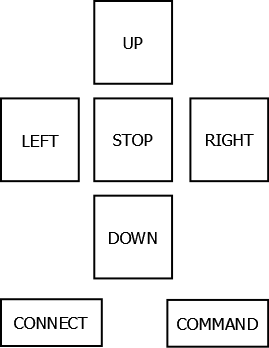
\includegraphics[scale=0.3]{img/styrkors}
                \caption{Styrning, uppkoppling \\ \& genväg till \ref{fig:command}}
                \label{fig:cross}
            \end{subfigure}
            \begin{subfigure}[b]{0.4\textwidth}
                \centering
                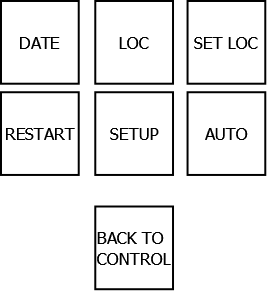
\includegraphics[scale=0.3]{img/command}
                \caption{Instruktion--gränssnittet \\ 'command'}
                \label{fig:command}
            \end{subfigure}
            \caption{Skiss av det grafiska gränssnittet}
        \end{figure}

        \paragraph{\textrm{Programmeringsspråk}} % (fold)
        \label{par:programmeringsspr_k}
            Den mjukvara som utvecklats till enheten är skrivet i programmeringsspråket \texttt{Python} och består av ett grafisk gränssnitt. Gränssnittet är uppdelat i två primära vyer, se figurerna \ref{fig:cross} och \ref{fig:command}, där de olika knapparna genererar de instruktioner som solpanelens styrkort lyssnar efter. \\

            \noindent Den första vyn som öppnas när applikationen start är den i \ref{fig:cross} och innehåller de grundläggande styrfunktionerna för justering av solpanelens rotering i X-- och Y--led. Knappen 'command' leder till den andra vyn som visas i figur \ref{fig:command}.
        % paragraph programmeringsspr_k (end)

   % section resultat (end)

    \newpage

    \section{Diskussion} % (fold)
    \label{sec:diskussion}
        \subsection{Hårdvara} % (fold)
        \label{sub:d_hardvara}
        
            Som nämnt på sidan \pageref{sub:beteckningar} så utgår vi ifrån begreppet enkortsdator för ett kretskort som är kapabel till att driva en Linuxkärna, till skillnad från en mikrokontroller där en svagare krets avses.\\

            \noindent Vår lösning är baserat på en enkortsdator och är fullt fungerande enligt de krav som uppdragsgivaren har fastställt och är relativt enkel att reproducera, i förhållande till att utveckla en likartad konstruktion med en mikrokontroller. Det som gör vår lösning enklare är fram för allt att en enkortsdator har de drivrutiner som krävs för att upprätta den seriella kommunikationen, så till vida att den har en Linuxkärna senare än version 3.0 \cite{silicon}. \\

            \noindent Nackdelar som vi ser med att använda en enkortsdator är bland andra att dessa generellt har ett större energibehov än en mikrokontroller \cite{gadgetBlog, rasp}. Antalet I/O portar är oftast färre på en enkortsdator och den fysiska storleken är större jämfört med de mikrokontrollerkort som hade varit lämpliga för projektet.\\

            \noindent Gällande frågeställningen om vår produkt är den enklaste att använda för kunderna, så ger vår produkt ett enkelt gränssnitt att använda, men en annan produkt med pekskärm kan komma att upplevas som lika enkelt. Vår produkt är något klumpig, vilket vi även påtalar i avsnitt \ref{subsub:val_av_plattform}, något som kan påverka användarvänligheten. En Androidenhet kan vara enklare att greppa om och visa upp samma gränssnitt, så ur en användares synsätt kan vår produkt inte vara den enklaste att nyttja, men ur en utvecklares perspektiv är det svårare att forma Android att göra det vi vill, så projektet kan ha resulterat utan någon produkt överhuvudtaget.

        % subsection h_rdvara (end)

        \subsection{Mjukvara} % (fold)
        \label{sub:d_mjukvara}

            Den mjukvara som har utvecklats, har skrivits i programmeringsspråket \texttt{Python}. Språk\-valet beror delvis på att personal inom företaget har erfarenhet inom språket vilket underlättar för framtida utveckling och underhåll av projektets produkt och dels valdes språket för dess enkla utveckling av grafiska gränssnitt och bra stöd i den seriella kommunikationen som krävdes i projektet. \\

            \noindent Andra språk som hade varit möjliga är till exempel \texttt{C} eller \texttt{Java} då projektgruppen har erfarenhet av de båda språken. \texttt{C} valdes bort då utveckling av grafiska gränssnitt i detta språk kräver externa bibliotek och minskar därför portabiliteten och ökar komplexiteten. \texttt{Java} är en lämplig kandidat för projektet, men valdes bort då den grafiska utvecklingen i \texttt{Python} är enklare och applikationen som vi utvecklade är såpass simpel att \texttt{Java} skulle medföra stor andel så kallad 'overhead' i programmeringskoden, något som visas när en jämförelse görs mellan de olika språken.\cite{Ferg}  Nackdelen med \texttt{Python} jämfört med \texttt{Java} är att språket inte är lika effektivt i sina beräkningar, men då applikationen vi skrivit inte utför några tyngre beräkningar så berörs inte användar\-upplevelsen  av detta. Kommer applikationen att vidareutvecklas till något mer än vad projektet skapat, är det fullt rimligt att översätta logiken till \texttt{Java}, något som det finns gott om stöd för.\cite{jython}
        % subsection mjukvara (end)
        
        \subsection{Framtida bruk} % (fold)
        \label{sub:framtida_bruk}
            Att projektet genomfördes grundar sig i SP3s bristande stöd för kommunikationsstandarder och att dagens kommunikationsgränssnitt inte är användarvänligt, vilket leder till stora underhållskostnader för företaget då det krävs tid och resurser att stötta underhålls\-personal. Detta projekt svarar upp på de förväntningar som bolaget hade på oss, men vi ser att projektets produkt kan komma att bli överflödig i nyare revisioner av panelen, där styrkortet kan ha tillgång till fler kommunikationsstandarder och kan komma att styras på distans.
        % subsection framtida_bruk (end)
    % section diskussion (end)

    \clearpage
    \addcontentsline{toc}{section}{Referenser}
    \printbibliography      
    
\end{document}
